% Auto-generated from docs/schematic/spec_protocol.py via render.py — edit the template, not the .tex.
\documentclass[tikz,border=6pt]{standalone}
\usepackage{amsmath}
\usepackage{tikz}
\usetikzlibrary{arrows.meta,calc,matrix}
\definecolor{plasticcol}{HTML}{4C8DFF}
\definecolor{frozencol}{HTML}{9AA0A6}
\definecolor{predcol}{HTML}{4C8DFF}
\definecolor{errcol}{HTML}{E0772B}
\definecolor{nodestroke}{HTML}{222222}
\definecolor{shadecol}{HTML}{3C4043}
\definecolor{clampcol}{HTML}{222222}
\definecolor{titlecol}{HTML}{222222}
\definecolor{mutedcol}{HTML}{6B7075}
% a small padlock at coordinate #1 in colour #2 — marks frozen weights
\newcommand{\padlock}[2]{%
  \begin{scope}[shift={#1}, draw=#2, line width=0.8pt, line join=round]
    \draw (-0.06,0.05) -- (-0.06,0.11) arc (180:0:0.06) -- (0.06,0.05); % shackle
    \fill[#2] (-0.11,-0.13) rectangle (0.11,0.05);                      % body
    \fill[white] (0,-0.03) circle (0.023);                             % keyhole
  \end{scope}}
\begin{document}
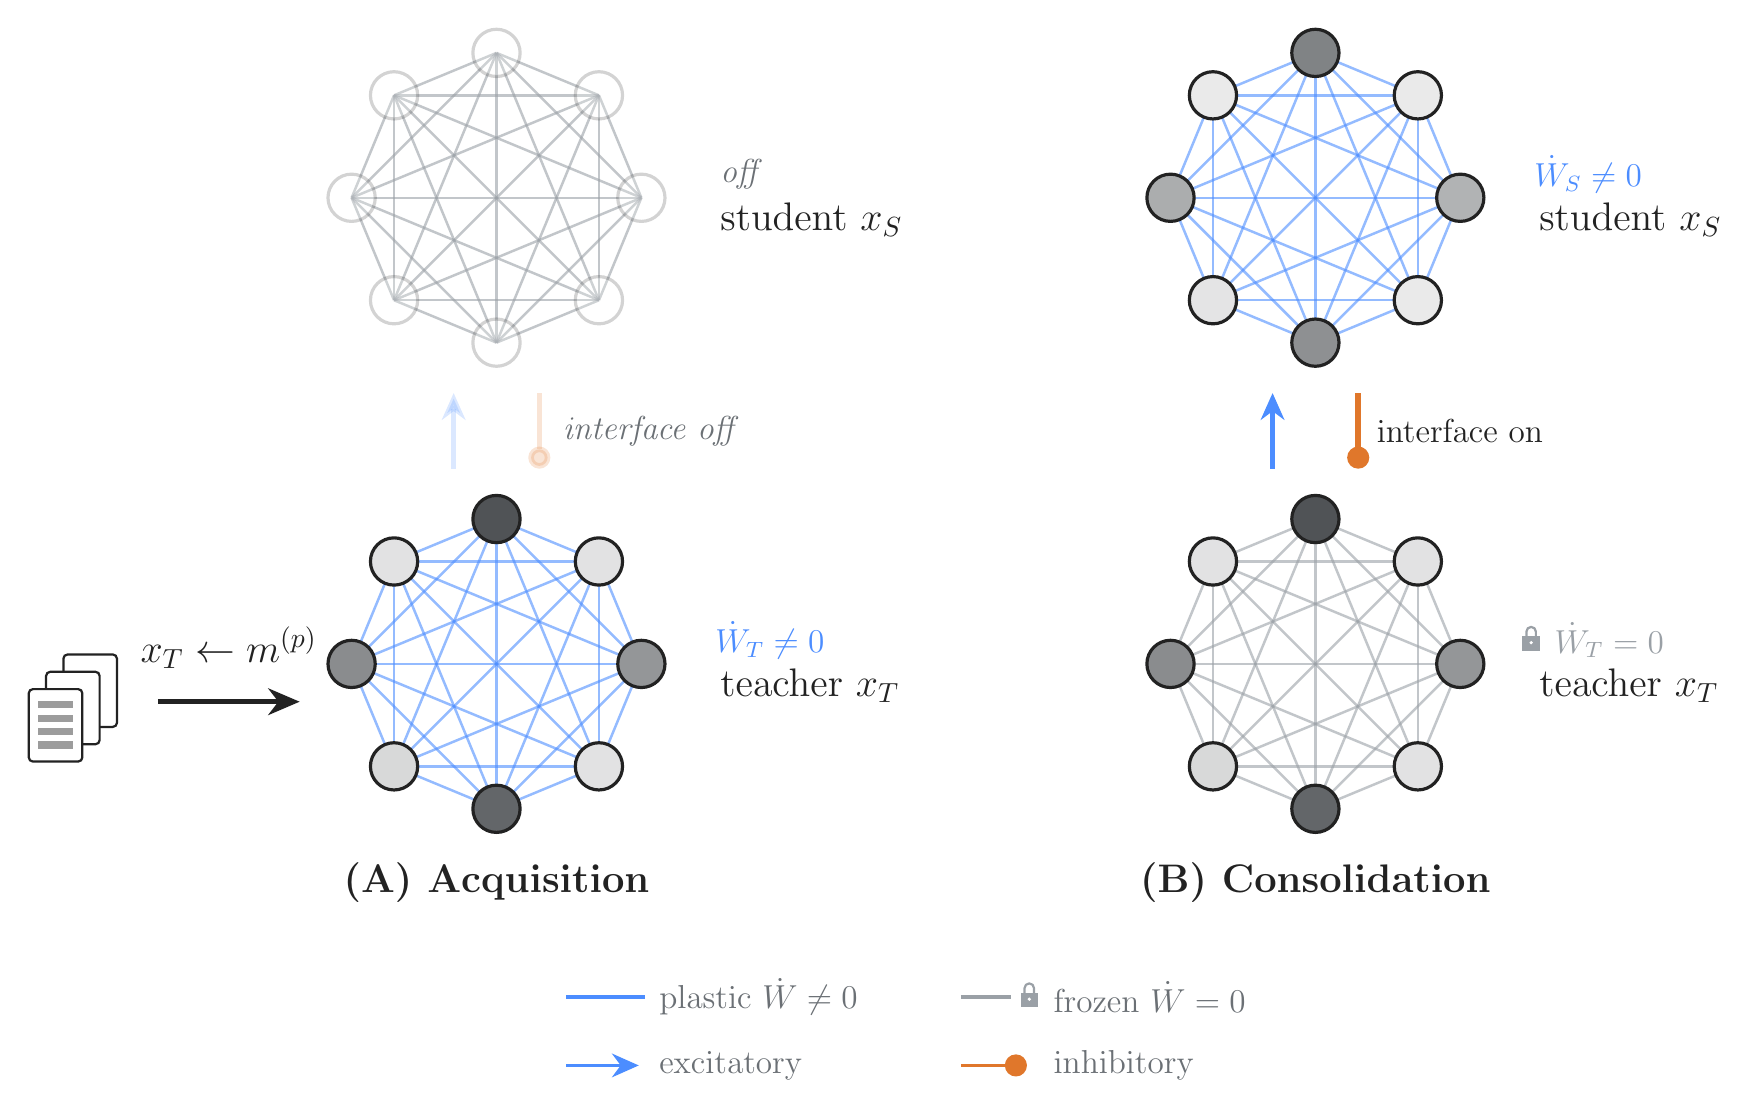
\begin{tikzpicture}[
  node/.style={circle, draw=nodestroke, line width=1.15pt, minimum size=6mm, inner sep=0pt},
  mesh/.style={line width=0.9pt, opacity=0.6},
  chord/.style={line width=1.35pt},
  interface/.style={line width=2pt},
  excit/.style={-{Stealth[length=3.4mm,width=3mm]}},
  inhib/.style={-{Circle[length=2.8mm, width=2.8mm]}},
  poplab/.style={font=\Large, text=titlecol},
  wlab/.style={font=\large, text=titlecol, fill=white, inner sep=1.5pt},
  offlab/.style={font=\large\itshape, text=mutedcol},
  title/.style={font=\Large\bfseries, text=titlecol},
  clab/.style={font=\large, text=clampcol, fill=white, inner sep=1.5pt},
  lgd/.style={font=\large, text=mutedcol},
]


% =================== PANEL A : Acquisition ===================

% ---- teacher ring (state: plastic) ----


% recurrent weights W_T: complete graph, drawn as a mesh BEHIND the nodes

\draw[mesh, plasticcol] (0.000,-4.080) -- (1.301,-4.619);

\draw[mesh, plasticcol] (0.000,-4.080) -- (1.840,-5.920);

\draw[mesh, plasticcol] (0.000,-4.080) -- (1.301,-7.221);

\draw[mesh, plasticcol] (0.000,-4.080) -- (0.000,-7.760);

\draw[mesh, plasticcol] (0.000,-4.080) -- (-1.301,-7.221);

\draw[mesh, plasticcol] (0.000,-4.080) -- (-1.840,-5.920);

\draw[mesh, plasticcol] (0.000,-4.080) -- (-1.301,-4.619);

\draw[mesh, plasticcol] (1.301,-4.619) -- (1.840,-5.920);

\draw[mesh, plasticcol] (1.301,-4.619) -- (1.301,-7.221);

\draw[mesh, plasticcol] (1.301,-4.619) -- (0.000,-7.760);

\draw[mesh, plasticcol] (1.301,-4.619) -- (-1.301,-7.221);

\draw[mesh, plasticcol] (1.301,-4.619) -- (-1.840,-5.920);

\draw[mesh, plasticcol] (1.301,-4.619) -- (-1.301,-4.619);

\draw[mesh, plasticcol] (1.840,-5.920) -- (1.301,-7.221);

\draw[mesh, plasticcol] (1.840,-5.920) -- (0.000,-7.760);

\draw[mesh, plasticcol] (1.840,-5.920) -- (-1.301,-7.221);

\draw[mesh, plasticcol] (1.840,-5.920) -- (-1.840,-5.920);

\draw[mesh, plasticcol] (1.840,-5.920) -- (-1.301,-4.619);

\draw[mesh, plasticcol] (1.301,-7.221) -- (0.000,-7.760);

\draw[mesh, plasticcol] (1.301,-7.221) -- (-1.301,-7.221);

\draw[mesh, plasticcol] (1.301,-7.221) -- (-1.840,-5.920);

\draw[mesh, plasticcol] (1.301,-7.221) -- (-1.301,-4.619);

\draw[mesh, plasticcol] (0.000,-7.760) -- (-1.301,-7.221);

\draw[mesh, plasticcol] (0.000,-7.760) -- (-1.840,-5.920);

\draw[mesh, plasticcol] (0.000,-7.760) -- (-1.301,-4.619);

\draw[mesh, plasticcol] (-1.301,-7.221) -- (-1.840,-5.920);

\draw[mesh, plasticcol] (-1.301,-7.221) -- (-1.301,-4.619);

\draw[mesh, plasticcol] (-1.840,-5.920) -- (-1.301,-4.619);


\node[node, fill=shadecol!90] (A-T0) at (0.000,-4.080) {};

\node[node, fill=shadecol!15] (A-T1) at (1.301,-4.619) {};

\node[node, fill=shadecol!55] (A-T2) at (1.840,-5.920) {};

\node[node, fill=shadecol!15] (A-T3) at (1.301,-7.221) {};

\node[node, fill=shadecol!80] (A-T4) at (0.000,-7.760) {};

\node[node, fill=shadecol!20] (A-T5) at (-1.301,-7.221) {};

\node[node, fill=shadecol!60] (A-T6) at (-1.840,-5.920) {};

\node[node, fill=shadecol!15] (A-T7) at (-1.301,-4.619) {};


% teacher recurrent-weight tag


\node[wlab, text=plasticcol, anchor=west] at (2.720,-5.620) {$\dot W_T\neq0$};

\node[poplab, anchor=west] at (2.720,-6.200) {teacher $x_T$};

% ---- student ring (state: off) ----

\begin{scope}[opacity=0.2]
% recurrent weights W_S: complete graph, drawn as a mesh BEHIND the nodes

\draw[mesh, frozencol] (0.000,1.840) -- (1.301,1.301);

\draw[mesh, frozencol] (0.000,1.840) -- (1.840,-0.000);

\draw[mesh, frozencol] (0.000,1.840) -- (1.301,-1.301);

\draw[mesh, frozencol] (0.000,1.840) -- (0.000,-1.840);

\draw[mesh, frozencol] (0.000,1.840) -- (-1.301,-1.301);

\draw[mesh, frozencol] (0.000,1.840) -- (-1.840,-0.000);

\draw[mesh, frozencol] (0.000,1.840) -- (-1.301,1.301);

\draw[mesh, frozencol] (1.301,1.301) -- (1.840,-0.000);

\draw[mesh, frozencol] (1.301,1.301) -- (1.301,-1.301);

\draw[mesh, frozencol] (1.301,1.301) -- (0.000,-1.840);

\draw[mesh, frozencol] (1.301,1.301) -- (-1.301,-1.301);

\draw[mesh, frozencol] (1.301,1.301) -- (-1.840,-0.000);

\draw[mesh, frozencol] (1.301,1.301) -- (-1.301,1.301);

\draw[mesh, frozencol] (1.840,-0.000) -- (1.301,-1.301);

\draw[mesh, frozencol] (1.840,-0.000) -- (0.000,-1.840);

\draw[mesh, frozencol] (1.840,-0.000) -- (-1.301,-1.301);

\draw[mesh, frozencol] (1.840,-0.000) -- (-1.840,-0.000);

\draw[mesh, frozencol] (1.840,-0.000) -- (-1.301,1.301);

\draw[mesh, frozencol] (1.301,-1.301) -- (0.000,-1.840);

\draw[mesh, frozencol] (1.301,-1.301) -- (-1.301,-1.301);

\draw[mesh, frozencol] (1.301,-1.301) -- (-1.840,-0.000);

\draw[mesh, frozencol] (1.301,-1.301) -- (-1.301,1.301);

\draw[mesh, frozencol] (0.000,-1.840) -- (-1.301,-1.301);

\draw[mesh, frozencol] (0.000,-1.840) -- (-1.840,-0.000);

\draw[mesh, frozencol] (0.000,-1.840) -- (-1.301,1.301);

\draw[mesh, frozencol] (-1.301,-1.301) -- (-1.840,-0.000);

\draw[mesh, frozencol] (-1.301,-1.301) -- (-1.301,1.301);

\draw[mesh, frozencol] (-1.840,-0.000) -- (-1.301,1.301);


\node[node, fill=shadecol!0] (A-S0) at (0.000,1.840) {};

\node[node, fill=shadecol!0] (A-S1) at (1.301,1.301) {};

\node[node, fill=shadecol!0] (A-S2) at (1.840,-0.000) {};

\node[node, fill=shadecol!0] (A-S3) at (1.301,-1.301) {};

\node[node, fill=shadecol!0] (A-S4) at (0.000,-1.840) {};

\node[node, fill=shadecol!0] (A-S5) at (-1.301,-1.301) {};

\node[node, fill=shadecol!0] (A-S6) at (-1.840,-0.000) {};

\node[node, fill=shadecol!0] (A-S7) at (-1.301,1.301) {};

\end{scope}
% student recurrent-weight tag


\node[offlab, anchor=west] at (2.720,0.300) {off};

\node[poplab, anchor=west] at (2.720,-0.280) {student $x_S$};

% ---- teacher <-> student interface (state: off) ----


\begin{scope}[opacity=0.2]
\draw[predcol, interface, excit] (-0.544,-3.440) -- (-0.544,-2.480);
\draw[errcol, interface, inhib] (0.544,-2.480) -- (0.544,-3.440);
\end{scope}
\node[offlab, anchor=west] at (0.720,-2.960) {interface off};


% ---- clamp x_T <- m^(p): a roomy stack of interleaved memory patterns + a bold arrow ----


% interleaved stack, back-to-front (offset up-right); front card carries a pattern hint
\foreach \d in {0.44,0.22,0}{
  \draw[clampcol, line width=0.8pt, fill=white, rounded corners=1.5pt]
     (-5.60+\d-0.34,-6.700+\d-0.46) rectangle (-5.60+\d+0.34,-6.700+\d+0.46);}
\foreach \k in {0.26,0.09,-0.08,-0.25}{
  \fill[clampcol!45] (-5.60-0.22,-6.700+\k-0.045) rectangle (-5.60+0.22,-6.700+\k+0.045);}
% bold clamp arrow into the teacher-left node
\draw[clampcol, line width=1.6pt, -{Stealth[length=4mm,width=3.4mm]}]
   (-4.3,-6.400) -- (-2.5,-6.400);
\node[font=\Large, text=clampcol, anchor=south] at (-3.4,-6.1) {$x_T\leftarrow m^{(p)}$};


% ---- panel title ----
\node[title, anchor=north] at (0.000,-8.320) {(A) Acquisition};

% =================== PANEL B : Consolidation ===================

% ---- teacher ring (state: frozen) ----


% recurrent weights W_T: complete graph, drawn as a mesh BEHIND the nodes

\draw[mesh, frozencol] (10.400,-4.080) -- (11.701,-4.619);

\draw[mesh, frozencol] (10.400,-4.080) -- (12.240,-5.920);

\draw[mesh, frozencol] (10.400,-4.080) -- (11.701,-7.221);

\draw[mesh, frozencol] (10.400,-4.080) -- (10.400,-7.760);

\draw[mesh, frozencol] (10.400,-4.080) -- (9.099,-7.221);

\draw[mesh, frozencol] (10.400,-4.080) -- (8.560,-5.920);

\draw[mesh, frozencol] (10.400,-4.080) -- (9.099,-4.619);

\draw[mesh, frozencol] (11.701,-4.619) -- (12.240,-5.920);

\draw[mesh, frozencol] (11.701,-4.619) -- (11.701,-7.221);

\draw[mesh, frozencol] (11.701,-4.619) -- (10.400,-7.760);

\draw[mesh, frozencol] (11.701,-4.619) -- (9.099,-7.221);

\draw[mesh, frozencol] (11.701,-4.619) -- (8.560,-5.920);

\draw[mesh, frozencol] (11.701,-4.619) -- (9.099,-4.619);

\draw[mesh, frozencol] (12.240,-5.920) -- (11.701,-7.221);

\draw[mesh, frozencol] (12.240,-5.920) -- (10.400,-7.760);

\draw[mesh, frozencol] (12.240,-5.920) -- (9.099,-7.221);

\draw[mesh, frozencol] (12.240,-5.920) -- (8.560,-5.920);

\draw[mesh, frozencol] (12.240,-5.920) -- (9.099,-4.619);

\draw[mesh, frozencol] (11.701,-7.221) -- (10.400,-7.760);

\draw[mesh, frozencol] (11.701,-7.221) -- (9.099,-7.221);

\draw[mesh, frozencol] (11.701,-7.221) -- (8.560,-5.920);

\draw[mesh, frozencol] (11.701,-7.221) -- (9.099,-4.619);

\draw[mesh, frozencol] (10.400,-7.760) -- (9.099,-7.221);

\draw[mesh, frozencol] (10.400,-7.760) -- (8.560,-5.920);

\draw[mesh, frozencol] (10.400,-7.760) -- (9.099,-4.619);

\draw[mesh, frozencol] (9.099,-7.221) -- (8.560,-5.920);

\draw[mesh, frozencol] (9.099,-7.221) -- (9.099,-4.619);

\draw[mesh, frozencol] (8.560,-5.920) -- (9.099,-4.619);


\node[node, fill=shadecol!90] (B-T0) at (10.400,-4.080) {};

\node[node, fill=shadecol!15] (B-T1) at (11.701,-4.619) {};

\node[node, fill=shadecol!55] (B-T2) at (12.240,-5.920) {};

\node[node, fill=shadecol!15] (B-T3) at (11.701,-7.221) {};

\node[node, fill=shadecol!80] (B-T4) at (10.400,-7.760) {};

\node[node, fill=shadecol!20] (B-T5) at (9.099,-7.221) {};

\node[node, fill=shadecol!60] (B-T6) at (8.560,-5.920) {};

\node[node, fill=shadecol!15] (B-T7) at (9.099,-4.619) {};


% teacher recurrent-weight tag


\padlock{ (13.140,-5.620) }{frozencol}
\node[wlab, text=frozencol, anchor=west] at (13.380,-5.620) {$\dot W_T=0$};

\node[poplab, anchor=west] at (13.120,-6.200) {teacher $x_T$};

% ---- student ring (state: plastic) ----


% recurrent weights W_S: complete graph, drawn as a mesh BEHIND the nodes

\draw[mesh, plasticcol] (10.400,1.840) -- (11.701,1.301);

\draw[mesh, plasticcol] (10.400,1.840) -- (12.240,-0.000);

\draw[mesh, plasticcol] (10.400,1.840) -- (11.701,-1.301);

\draw[mesh, plasticcol] (10.400,1.840) -- (10.400,-1.840);

\draw[mesh, plasticcol] (10.400,1.840) -- (9.099,-1.301);

\draw[mesh, plasticcol] (10.400,1.840) -- (8.560,-0.000);

\draw[mesh, plasticcol] (10.400,1.840) -- (9.099,1.301);

\draw[mesh, plasticcol] (11.701,1.301) -- (12.240,-0.000);

\draw[mesh, plasticcol] (11.701,1.301) -- (11.701,-1.301);

\draw[mesh, plasticcol] (11.701,1.301) -- (10.400,-1.840);

\draw[mesh, plasticcol] (11.701,1.301) -- (9.099,-1.301);

\draw[mesh, plasticcol] (11.701,1.301) -- (8.560,-0.000);

\draw[mesh, plasticcol] (11.701,1.301) -- (9.099,1.301);

\draw[mesh, plasticcol] (12.240,-0.000) -- (11.701,-1.301);

\draw[mesh, plasticcol] (12.240,-0.000) -- (10.400,-1.840);

\draw[mesh, plasticcol] (12.240,-0.000) -- (9.099,-1.301);

\draw[mesh, plasticcol] (12.240,-0.000) -- (8.560,-0.000);

\draw[mesh, plasticcol] (12.240,-0.000) -- (9.099,1.301);

\draw[mesh, plasticcol] (11.701,-1.301) -- (10.400,-1.840);

\draw[mesh, plasticcol] (11.701,-1.301) -- (9.099,-1.301);

\draw[mesh, plasticcol] (11.701,-1.301) -- (8.560,-0.000);

\draw[mesh, plasticcol] (11.701,-1.301) -- (9.099,1.301);

\draw[mesh, plasticcol] (10.400,-1.840) -- (9.099,-1.301);

\draw[mesh, plasticcol] (10.400,-1.840) -- (8.560,-0.000);

\draw[mesh, plasticcol] (10.400,-1.840) -- (9.099,1.301);

\draw[mesh, plasticcol] (9.099,-1.301) -- (8.560,-0.000);

\draw[mesh, plasticcol] (9.099,-1.301) -- (9.099,1.301);

\draw[mesh, plasticcol] (8.560,-0.000) -- (9.099,1.301);


\node[node, fill=shadecol!65] (B-S0) at (10.400,1.840) {};

\node[node, fill=shadecol!11] (B-S1) at (11.701,1.301) {};

\node[node, fill=shadecol!40] (B-S2) at (12.240,-0.000) {};

\node[node, fill=shadecol!11] (B-S3) at (11.701,-1.301) {};

\node[node, fill=shadecol!58] (B-S4) at (10.400,-1.840) {};

\node[node, fill=shadecol!14] (B-S5) at (9.099,-1.301) {};

\node[node, fill=shadecol!43] (B-S6) at (8.560,-0.000) {};

\node[node, fill=shadecol!11] (B-S7) at (9.099,1.301) {};


% student recurrent-weight tag


\node[wlab, text=plasticcol, anchor=west] at (13.120,0.300) {$\dot W_S\neq0$};

\node[poplab, anchor=west] at (13.120,-0.280) {student $x_S$};

% ---- teacher <-> student interface (state: on) ----



\draw[predcol, interface, excit] (9.856,-3.440) -- (9.856,-2.480);
\draw[errcol, interface, inhib] (10.944,-2.480) -- (10.944,-3.440);

\node[wlab, anchor=west] at (11.120,-2.960) {interface on};


% ---- clamp x_T <- m^(p): a roomy stack of interleaved memory patterns + a bold arrow ----


% ---- panel title ----
\node[title, anchor=north] at (10.400,-8.320) {(B) Consolidation};


% =================== legend (matrix measures text widths and spaces entries evenly) ===================

\matrix (legend) [
  matrix of nodes,
  anchor=center,
  nodes={anchor=west, inner sep=0pt, outer sep=0pt},
  column sep=0.18cm,
  row sep=0.45cm
] at (5.200,-10.560) {
  |[minimum width=1.0cm, minimum height=0.32cm]| {} &
  |[lgd]| {plastic $\dot W\neq0$} &
  |[minimum width=0.95cm]| {} &
  |[minimum width=1.0cm, minimum height=0.32cm]| {} &
  |[lgd]| {frozen $\dot W=0$} \\
  |[minimum width=1.0cm, minimum height=0.32cm]| {} &
  |[lgd]| {excitatory} &
  |[minimum width=0.95cm]| {} &
  |[minimum width=1.0cm, minimum height=0.32cm]| {} &
  |[lgd]| {inhibitory} \\
};
\draw[plasticcol, chord] (legend-1-1.west) -- (legend-1-1.east);
\draw[frozencol, chord] (legend-1-4.west) -- ($(legend-1-4.east)+(-0.36,0)$);
\coordinate (legend-lock) at ($(legend-1-4.east)+(-0.13,0)$);
\padlock{(legend-lock)}{frozencol}
\draw[predcol, chord, excit] (legend-2-1.west) -- ($(legend-2-1.east)+(-0.08,0)$);
\draw[errcol, chord, inhib] (legend-2-4.west) -- ($(legend-2-4.east)+(-0.16,0)$);
\end{tikzpicture}
\end{document}